\documentclass[11pt]{article}

\usepackage[T1]{fontenc}
\usepackage[utf8]{inputenc}
\usepackage[scaled=0.94]{helvet}
\renewcommand{\familydefault}{\sfdefault}
\usepackage{microtype}
\usepackage[a4paper,margin=19mm,headheight=15pt,footskip=24pt]{geometry}
\usepackage[table]{xcolor}
\usepackage{graphicx}
\usepackage{booktabs}
\usepackage{array}
\usepackage{tabularx}
\usepackage{longtable}
\usepackage{longtable-finite-glue}
\usepackage{enumitem}
\usepackage{listings}
\usepackage[most]{tcolorbox}
\usepackage{tikz}
\usetikzlibrary{positioning}
\usepackage{titlesec}
\usepackage{fancyhdr}
\usepackage{lastpage}
\usepackage{hyperref}
\usepackage{pifont}

\definecolor{Ink}{HTML}{111827}
\definecolor{Navy}{HTML}{090A1A}
\definecolor{DeepBlue}{HTML}{102A56}
\definecolor{Electric}{HTML}{00D69C}
\definecolor{Cyan}{HTML}{23C9E8}
\definecolor{Magenta}{HTML}{EF4CCB}
\definecolor{Warning}{HTML}{B42318}
\definecolor{Gold}{HTML}{B7791F}
\definecolor{Muted}{HTML}{5F6B7A}
\definecolor{Rule}{HTML}{D6DEE8}
\definecolor{Paper}{HTML}{F5F8FB}
\definecolor{PaleGreen}{HTML}{EAFBF5}
\definecolor{PaleBlue}{HTML}{EAF7FC}
\definecolor{PaleRed}{HTML}{FFF1F0}
\definecolor{PaleGold}{HTML}{FFF8E8}

\hypersetup{%
  colorlinks=true,
  linkcolor=DeepBlue,
  urlcolor=DeepBlue,
  pdftitle={DOGFOOD 2026 Participant Handbook and Technical Brief},
  pdfauthor={Prepared from the DOGFOOD 2026 kickoff deck},
  pdfsubject={Comprehensive hackathon requirements, judging, delivery, and implementation guide}
}

\setlength{\parindent}{0pt}
\setlength{\parskip}{5pt}
\raggedbottom{}
\setlist[itemize]{leftmargin=5mm,itemsep=2pt,topsep=3pt}
\setlist[enumerate]{leftmargin=6mm,itemsep=2pt,topsep=3pt}
\renewcommand{\arraystretch}{1.22}

\newcolumntype{Y}{>{\raggedright\arraybackslash}X}
\newcolumntype{L}[1]{>{\raggedright\arraybackslash}p{#1}}
\newcommand{\yes}{\textcolor{Electric!70!black}{\ding{51}}}
\newcommand{\no}{\textcolor{Warning}{\ding{55}}}
\newcommand{\checkbox}{\textcolor{DeepBlue}{\ding{113}}}
\newcommand{\term}[1]{\textbf{\textcolor{DeepBlue}{#1}}}
\newcommand{\official}{\textcolor{Electric!60!black}{\textbf{OFFICIAL REQUIREMENT}}}
\newcommand{\advisory}{\textcolor{DeepBlue}{\textbf{IMPLEMENTATION GUIDANCE}}}
\newcommand{\rr}[1]{\textsuperscript{\textcolor{DeepBlue}{[#1]}}}

\titleformat{\section}{\Large\bfseries\color{Navy}}{\thesection}{0.55em}{}[\vspace{2pt}\color{Electric}\titlerule]
\titleformat{\subsection}{\large\bfseries\color{DeepBlue}}{\thesubsection}{0.5em}{}
\titleformat{\subsubsection}{\normalsize\bfseries\color{Ink}}{}{0pt}{}
\titlespacing*{\section}{0pt}{18pt}{8pt}
\titlespacing*{\subsection}{0pt}{13pt}{5pt}

\pagestyle{fancy}
\fancyhf{}
\fancyhead[L]{\small\textbf{DOGFOOD 2026}}
\fancyhead[R]{\small Participant Handbook \& Technical Brief}
\fancyfoot[L]{\scriptsize Build the Platform That Will Judge You}
\fancyfoot[R]{\scriptsize Page~\thepage\ of~\pageref*{LastPage}}
\renewcommand{\headrulewidth}{0.4pt}
\renewcommand{\footrulewidth}{0.4pt}

\newtcolorbox{keybox}[1][]{%
  breakable,colback=PaleGreen,colframe=Electric!65!black,boxrule=0.8pt,
  arc=2mm,left=4mm,right=4mm,top=3mm,bottom=3mm,#1
}
\newtcolorbox{infobox}[1][]{%
  breakable,colback=PaleBlue,colframe=Cyan!70!black,boxrule=0.8pt,
  arc=2mm,left=4mm,right=4mm,top=3mm,bottom=3mm,#1
}
\newtcolorbox{warningbox}[1][]{%
  breakable,colback=PaleRed,colframe=Warning,boxrule=0.8pt,
  arc=2mm,left=4mm,right=4mm,top=3mm,bottom=3mm,#1
}
\newtcolorbox{advicebox}[1][]{%
  breakable,colback=PaleGold,colframe=Gold,boxrule=0.8pt,
  arc=2mm,left=4mm,right=4mm,top=3mm,bottom=3mm,#1
}

\lstdefinestyle{dogfood}{%
  backgroundcolor=\color{Navy},
  basicstyle=\ttfamily\small\color{white},
  keywordstyle=\color{Electric},
  commentstyle=\color{Cyan},
  stringstyle=\color{white},
  frame=single,
  rulecolor=\color{DeepBlue},
  frameround=tttt,
  xleftmargin=2mm,
  xrightmargin=2mm,
  aboveskip=6pt,
  belowskip=6pt,
  breaklines=true,
  showstringspaces=false,
  columns=fullflexible
}

\begin{document}
\pagenumbering{roman}

% -----------------------------------------------------------------------------
% Cover
% -----------------------------------------------------------------------------
\begin{titlepage}
\pagecolor{Navy}
\color{white}
\begin{tikzpicture}[remember picture,overlay]
  \fill[DeepBlue] (current page.north west) rectangle ([xshift=-0.46\paperwidth]current page.south east);
  \foreach \x/\y/\r in {2/3/0.9,5/7/1.3,9/2/0.7,12/9/1.0,15/5/0.6}{%
    \draw[Electric,opacity=.35,line width=.8pt] ([xshift=\x cm,yshift=-\y cm]current page.north west) circle (\r cm);
  }
  \draw[Cyan,opacity=.30,line width=1pt]
    ([xshift=11cm,yshift=-4cm]current page.north west) --
    ([xshift=15cm,yshift=-7cm]current page.north west) --
    ([xshift=12cm,yshift=-11cm]current page.north west) --
    ([xshift=17cm,yshift=-15cm]current page.north west);
  \draw[Magenta,opacity=.25,line width=1pt]
    ([xshift=8cm,yshift=-20cm]current page.north west) --
    ([xshift=13cm,yshift=-17cm]current page.north west) --
    ([xshift=18cm,yshift=-21cm]current page.north west);
  \fill[Electric] ([xshift=18mm,yshift=18mm]current page.south west) rectangle ([xshift=24mm,yshift=20mm]current page.south west);
\end{tikzpicture}

\vspace*{22mm}
{\fontsize{38}{42}\selectfont\bfseries DOGFOOD}\par
\vspace{3mm}
{\LARGE\bfseries 2026 Participant Handbook}\par
{\LARGE\bfseries \& Technical Brief}\par

\vspace{11mm}
{\large Build the Platform That Will Judge You}\par
\vspace{3mm}
{\normalsize A comprehensive interpretation of the kickoff deck, including every stated requirement, check, deliverable, scoring rule, deadline, prize, and adoption term.}\par

\vfill
\begin{tcolorbox}[colback=DeepBlue,coltext=white,fontupper=\color{white},colframe=Electric,boxrule=1pt,arc=2mm,left=5mm,right=5mm,top=4mm,bottom=4mm]
\begin{tabularx}{\linewidth}{@{}Y Y@{}}
\textbf{Event} & September 26--29, 2026\\
\textbf{Format} & Online, free to enter\\
\textbf{Prize pool} & \$2,500\\
\textbf{Primary output} & A working, open-source hackathon portal\\
\textbf{Run requirement} & \texttt{docker compose up}, offline\\
\textbf{Document date} & September 27, 2026\\
\end{tabularx}
\end{tcolorbox}

\vspace{8mm}
{\small Prepared from \texttt{prism-uploads/Copy-of-DogFood-2026-Kickoff.pdf}. Where this handbook offers design advice beyond the deck, it is explicitly labeled as guidance rather than an official rule.}\par
\end{titlepage}
\pagenumbering{arabic}
\nopagecolor{}
\color{Ink}

\begin{keybox}[title=\textbf{Status on September 27, 2026}]
The hacking window is currently open. It began on September 26 at 18:00 UTC\@. and closes on September 29 at 18:00 UTC\@. The next hard milestone is the code freeze and submission deadline on September 29 at 18:00 UTC\@.
\end{keybox}

\tableofcontents
\clearpage

% -----------------------------------------------------------------------------
\section{Executive understanding}

DOGFOOD is not a conventional ideation contest. It is an open commissioning exercise: the organizers want participants to build the hackathon submission and judging platform that will replace the inadequate tools currently available. The winning project is intended to be forked, self-hosted, and used for future events.

The expected product is a complete portal that an organizer could operate immediately after the event. It must cover the lifecycle from registration and team formation through submission, eligibility, judge assignment, scoring, normalization, results, and export. It must be operational software rather than a mockup, isolated feature, design system, or slide deck.

\begin{keybox}
\textbf{The central success criterion:} produce a trustworthy, adoptable system in which judging is correct, transparent, secure, and operable. Feature breadth matters only after the foundational workflows work cleanly.
\end{keybox}

\subsection{The non-negotiable shape of the solution}

\begin{itemize}
  \item One integrated product, not separate gallery and judging demonstrations.
  \item A seeded portal that starts with \texttt{docker compose up}.
  \item Functional on a laptop with the network disconnected.
  \item Open source under an OSI-approved license.
  \item Backend-enforced authorization, especially around private judge scores.
  \item Honest tier claims and an acceptance report committed even when checks fail.
  \item Documentation that explains the architecture, schema, judging mathematics, limitations, and operating procedure.
\end{itemize}

\subsection{Event snapshot}

\rowcolors{2}{Paper}{white}
\begin{tabularx}{\linewidth}{@{}L{40mm}Y@{}}
\toprule
\textbf{Item} & \textbf{Official detail}\\
\midrule
Name & DOGFOOD\@: Build the Platform That Will Judge You\\
Dates & September 26--29, 2026\\
Format & Online\\
Entry fee & Free\\
Prize pool & \$2,500\\
Hacking window & September 26, 18:00 UTC to September 29, 18:00 UTC\\
Judging window & September 29 through October 8, asynchronously, with multiple judges per project\\
Winner announcement & October 9, 2026\\
Primary adoption promise & The organizers will fork, self-host, and run the winning platform\\
\bottomrule
\end{tabularx}

% -----------------------------------------------------------------------------
\section{The problem statement}

The kickoff deck argues that mainstream hackathon platforms converged on roughly the same feature set and then stopped improving. The challenge targets four specific structural failures.

\subsection{Broken judging}

The category leader cannot weight judging criteria. Its own documentation reportedly directs organizers to conduct judging outside the platform in a spreadsheet. This fragments the process, weakens auditability, creates manual transfer risk, and makes the central activity of the event dependent on tooling outside the event platform.

\subsection{Opaque normalization}

Several platforms advertise automatic score normalization without explaining the method. A result can therefore look mathematically authoritative without allowing organizers, judges, or participants to understand how raw scores became rankings. DOGFOOD expects the method to be explicit and defended.

\subsection{Gameable community voting}

Community voting is treated across the industry as vulnerable to manipulation. The common workaround is to reduce the value of the prize and hide interim results rather than solve the underlying abuse problem. DOGFOOD asks higher-tier entries to build voting controls and preserve an audit trail.

\subsection{No public API}

After many years and millions of participating developers, the established platforms still do not provide a usable public API\@. Organizers integrate through scraping and downloaded CSV files. The stretch tier challenges entrants to make the platform programmable through a REST API, webhooks, and comprehensive import/export.

\begin{infobox}
\textbf{Problem in one sentence:} hackathon platforms handle the visible surface of events but fail at transparent, secure, extensible judging---the part participants ultimately depend on.
\end{infobox}

% -----------------------------------------------------------------------------
\section{Mission and definition of done}

\official\par


Build a hackathon submission and judging portal that an organizer could run on Monday. It must be working software, not a mockup, design system, or presentation.

\subsection{The end-to-end lifecycle}

The mission slide calls the workflow ``ten stages'' but explicitly names nine. The named stages are shown below. Event creation, which is explicitly required in Tier 1, is the most plausible implicit tenth stage; however, the source deck does not formally resolve the discrepancy.

\rowcolors{2}{Paper}{white}
\begin{tabularx}{\linewidth}{@{}L{9mm}L{37mm}Y@{}}
\toprule
\textbf{No.} & \textbf{Stage} & \textbf{Expected product behavior}\\
\midrule
1 & Registration & Establish participant identity and access to the event.\\
2 & Teams & Form and manage teams participating in the event.\\
3 & Submissions & Create and update projects, then enforce the final submission window.\\
4 & Eligibility & Determine whether a participant or project may proceed to judging.\\
5 & Judge assignment & Invite judges and allocate projects or review batches.\\
6 & Scoring & Capture scores through a weighted rubric.\\
7 & Normalization & Make scores from differently calibrated judges comparable.\\
8 & Results & Produce rankings and control when results become visible.\\
9 & Export & Provide machine-readable data, at minimum the required CSV export.\\
--- & Implicit enabler & Event creation is a Tier 1 requirement and may account for the deck's stated tenth stage.\\
\bottomrule
\end{tabularx}

Each stage feeds the next. A defect in registration, eligibility, assignment, or scoring ultimately damages judging, even when the defect appears earlier in the workflow.

\subsection{Operational acceptance}

The required invocation is deliberately simple:

\begin{lstlisting}[style=dogfood]
docker compose up
\end{lstlisting}

After that command, the portal must be seeded and usable on a laptop without network access. A solution that depends on a cloud database, hosted authentication service, or external account cannot be adopted and is explicitly out of scope.

% -----------------------------------------------------------------------------
\section{The four-tier ladder}

There are no separate tracks. Every team builds the same class of product and progresses through four cumulative tiers. Advancement depends on how far the team gets and how cleanly each tier works.

\begin{keybox}
\textbf{Priority rule:} a clean Tier 2 beats a broken Tier 4. Correctness outranks breadth.
\end{keybox}

\subsection{Tier 1---Core: the mandatory floor}

Tier 1 must be cleared or the entry is not judged. It includes:

\begin{itemize}
  \item authentication;
  \item roles;
  \item event creation;
  \item team formation;
  \item project submission;
  \item deadline enforcement; and
  \item a public project gallery.
\end{itemize}

This tier establishes that the entry is an actual event portal rather than a judging prototype or gallery mockup.

\subsection{Tier 2---Judging: the central engineering tier}

Tier 2 contains the capabilities the challenge is chiefly designed to improve:

\begin{itemize}
  \item judge invitation and assignment;
  \item a weighted scoring rubric;
  \item role isolation enforced in the backend;
  \item a judging progress dashboard;
  \item cross-judge score normalization; and
  \item CSV export.
\end{itemize}

Tier 2 is both technically consequential and heavily aligned with the scoring rubric: judging integrity alone contributes 25\% of the weighted score.

\subsection{Tier 3---Public participation}

Tier 3 adds public-facing interaction while requiring controls against premature disclosure and manipulation:

\begin{itemize}
  \item community voting;
  \item comments;
  \item results hidden until the voting or judging window closes;
  \item randomized ballot order; and
  \item anti-abuse controls with an audit trail.
\end{itemize}

\subsection{Tier 4---Stretch and ecosystem}

Tier 4 turns the portal into a broader platform:

\begin{itemize}
  \item REST API with webhooks;
  \item certificates;
  \item verifiable judge records;
  \item an embeddable project gallery; and
  \item bulk import and export.
\end{itemize}

\subsection{Dependency logic}

\begin{tabularx}{\linewidth}{@{}L{27mm}Y Y@{}}
\toprule
\textbf{Tier} & \textbf{Depends on} & \textbf{Primary failure to avoid}\\
\midrule
T1 & Local runtime, identities, event state, seed data & A product that looks complete but cannot run or enforce deadlines\\
T2 & Correct T1 entities and permissions & Score leakage, incorrect assignments, unexplained rankings\\
T3 & Stable project/result models and auditable identity & Ballot stuffing, order bias, early result disclosure\\
T4 & Stable domain model and service boundaries & An API that exposes inconsistent or insecure behavior\\
\bottomrule
\end{tabularx}

% -----------------------------------------------------------------------------
\section{The acceptance checker}

\official\par


The organizers provide one Python file using only the standard library. Every team runs the same checker, which reduces subjective variation in how the foundational tiers are verified.

\begin{lstlisting}[style=dogfood]
python3 run.py ".dogfood.toml"
\end{lstlisting}

The checker performs seven tests: three for Tier 1 and four for Tier 2. Tiers 3 and 4 are judged manually.

\subsection{All seven machine checks}

\rowcolors{2}{Paper}{white}
\begin{longtable}{@{}L{13mm}L{45mm}L{31mm}L{70mm}@{}}
\toprule
\textbf{Tier} & \textbf{Check} & \textbf{Area} & \textbf{Meaning}\\
\midrule
\endhead%
T1 & Gallery is public & Public access & An unauthenticated visitor can reach the configured gallery.\\
T1 & Fixture projects shown & Seed integrity & The shared fixture projects are present in the gallery.\\
T1 & Closed event refuses submissions & Deadline enforcement & A project cannot be submitted after the fixture event's submission close time.\\
T2 & Judge sees own scores & Authorized access & A judge can retrieve the scores that belong to that judge.\\
T2 & Judge cannot see peer scores & Role isolation & A judge cannot retrieve another judge's private scores.\\
T2 & Participant blocked & Role isolation & A participant is denied access to judge-only scoring data or behavior.\\
T2 & CSV export works & Portability & The configured export route returns a functioning CSV export.\\
\bottomrule
\end{longtable}

The deck does not publish every assertion or response format on the slide itself. Entrants are explicitly told to read \texttt{run.py}, because that file is the definitive description of the automated behavior.

\subsection{Configuration through \texttt{.dogfood.toml}}

The repository root must contain a short TOML file, described as approximately six to fifteen lines in ordinary use. Teams may choose their own route names and authentication mechanism, then tell the checker where those capabilities live.

\begin{lstlisting}[style=dogfood]
[portal]
base_url = "http://localhost:8080"

[tiers]
claimed = ["T1", "T2"]

[auth]
organizer   = "Cookie: session=org_7f2a"
judge_a     = "Cookie: session=jdg_a_91bc"
judge_b     = "Cookie: session=jdg_b_44de"
participant = "Cookie: session=prt_2e88"

[routes]
gallery      = "/projects"
submit       = "/projects/new"
judge_scores = "/api/judge/scores"
peer_scores  = "/api/judge/scores?judge=judge_a"
csv_export   = "/api/export.csv"
\end{lstlisting}

The checker does not perform an interactive login. The team supplies working authorization headers, and the checker attaches the appropriate header to each request. Consequently, the login page and session-creation flow may be implemented in any reasonable way, while the checker receives ready-to-use credentials.

\subsection{Acceptance-report discipline}

Teams are told to run the checker early and repeatedly, then commit its output regardless of whether every line passes. Two honest failures are considered more credible than a README that claims unsupported completeness. This rule reinforces the scoring policy that rewards honest gaps and penalizes inflated claims.

% -----------------------------------------------------------------------------
\section{The shared fixture dataset}

Every team receives and loads the same \texttt{fixtures.json}. It contains:

\begin{itemize}
  \item 40 projects;
  \item 30 judges;
  \item 8 tracks; and
  \item a complete collection of scores.
\end{itemize}

The fixture data uses no real names. It intentionally includes awkward operational cases:

\begin{itemize}
  \item one judge who assigned the same score to everything;
  \item two review batches that were never completed; and
  \item a duplicate submission.
\end{itemize}

These are not accidental dirty-data problems. They are deliberate probes of how the platform behaves under conditions that occur in real hackathons.

\begin{warningbox}
\textbf{Date-sensitive requirement:} seed the event using the fixture event's own \texttt{submissions\_close} value. One of the acceptance checks depends on that timestamp. Replacing it with ``now plus three days'' or another generated value can cause the deadline test to fail.
\end{warningbox}

The fixture data, specification, and checker were described as already downloadable from the specification site at kickoff; no additional hidden file is expected to appear later.

\subsection{What the edge cases imply}

\advisory\par


\begin{itemize}
  \item A constant-scoring judge creates zero variance, which must be handled explicitly by any variance-based normalization method.
  \item Incomplete batches require visible progress states and a policy for rankings produced before all reviews are complete.
  \item A duplicate submission should not silently distort assignments, voting, or rankings. The product should identify, reject, merge, or clearly flag it.
  \item Seed logic should be repeatable so evaluators can recreate a known state without manually repairing duplicates.
\end{itemize}

% -----------------------------------------------------------------------------
\section{The critical authorization requirement}

The deck singles out one check as the most common and expensive failure:

\begin{keybox}
\textbf{A judge must not be able to read another judge's scores---not through the user interface and not through the API.}
\end{keybox}

The checker authenticates as \texttt{judge\_b} and calls the route that identifies \texttt{judge\_a}'s scores. A \texttt{200} response fails the check. The response must be \texttt{401 Unauthorized} or \texttt{403 Forbidden}.

Hiding a button is not authorization. A user can bypass the interface with an HTTP client such as \texttt{curl}. The ownership or role check must execute on the server before score data is read or returned.

\subsection{Suggested authorization matrix}

\advisory\par


The following matrix is not prescribed by the deck, but it is a practical way to reason about the required isolation.

\begin{tabularx}{\linewidth}{@{}L{29mm}Y Y Y Y@{}}
\toprule
\textbf{Action} & \textbf{Anonymous} & \textbf{Participant} & \textbf{Judge} & \textbf{Organizer}\\
\midrule
View public gallery & Allow & Allow & Allow & Allow\\
Submit before deadline & Deny & Own team only & Deny unless separately eligible & Administrative access\\
Read own judge scores & Deny & Deny & Allow own only & Allow if policy permits\\
Read peer judge scores & Deny & Deny & Deny & Allow only if required operationally\\
Assign projects & Deny & Deny & Deny & Allow\\
Publish results & Deny & Deny & Deny & Allow after appropriate window\\
Export event data & Deny & Deny & Usually deny & Allow\\
\bottomrule
\end{tabularx}

The authorization check should use the authenticated server-side identity, not a judge identifier supplied by the request. Query parameters can select a resource, but they must never grant ownership.

% -----------------------------------------------------------------------------
\section{Submission package: everything that must ship}

The deck defines nine deliverables.

\begin{longtable}{@{}L{9mm}L{43mm}L{105mm}@{}}
\toprule
\textbf{No.} & \textbf{Deliverable} & \textbf{Required content or behavior}\\
\midrule
\endhead%
1 & Public GitHub repository & Public source with an OSI-approved license. MIT or Apache-2.0 is preferred.\\
2 & \texttt{docker compose up} & Starts a seeded, working portal that remains usable without network access.\\
3 & \texttt{.dogfood.toml} & Lives at the repository root and declares routes, auth headers, base URL, and honest tier claims.\\
4 & \texttt{acceptance-report.txt} & The checker's actual output, committed regardless of pass or fail.\\
5 & \texttt{README.md} & Explains what the product does, how to run it, and its honest limitations.\\
6 & \texttt{ARCHITECTURE.md} & Describes the system's shape and the reasoning behind it.\\
7 & \texttt{DATA-MODEL.md} & Documents the schema and the import/export pathways.\\
8 & \texttt{JUDGING.md} & Defends the assignment strategy, scoring mathematics, and normalization method.\\
9 & Five-minute demo video & Demonstrates one complete event lifecycle.\\
\bottomrule
\end{longtable}

\begin{warningbox}
\textbf{Documentation is scored work, not packaging overhead.} \texttt{JUDGING.md} feeds directly into the 25\% Judging Integrity category. ``We averaged the scores'' is technically an answer, but the deck explicitly describes it as a weak one.
\end{warningbox}

\subsection{What a strong five-minute demonstration should establish}

\advisory\par


To show a full lifecycle within five minutes, a concise sequence would be:

\begin{enumerate}
  \item start the seeded system locally;
  \item show the public gallery and fixture projects;
  \item create or inspect an event and its submission deadline;
  \item demonstrate a participant submission before or after the appropriate deadline;
  \item assign a project to a judge;
  \item enter weighted scores;
  \item prove that a second judge cannot access the first judge's scores;
  \item show judging progress and normalized results;
  \item export CSV\@; and
  \item show the acceptance report and honestly state remaining gaps.
\end{enumerate}

% -----------------------------------------------------------------------------
\section{Scoring model}

The weighted evaluation is:

\begin{tabularx}{\linewidth}{@{}L{30mm}L{55mm}Y@{}}
\toprule
\textbf{Weight} & \textbf{Category} & \textbf{What it rewards}\\
\midrule
40\% & Tier Completion \& Correctness & How far the product progresses while keeping claimed functionality correct\\
25\% & Judging Integrity & Assignment quality, scoring design, authorization, normalization, and defensibility\\
20\% & Adoptability \& Operability & Offline startup, clear setup, documentation, maintainability, and practical event operation\\
15\% & Code Quality \& Innovation & Engineering quality and meaningful new capability\\
\bottomrule
\end{tabularx}

Tier 1 is a gate rather than a source of points: failure to clear it means the entry is not judged. Above that floor, correctness is more valuable than claiming additional tiers with partially working functionality.

\begin{keybox}
Honest gap reporting is rewarded. Inflated claims are penalized.
\end{keybox}

\subsection{Practical scoring implications}

\advisory\par


\begin{itemize}
  \item Do not sacrifice T1 reliability for a stretch feature; T1 controls eligibility for judging.
  \item Prioritize backend authorization, scoring, and normalization because they affect both tier completion and judging integrity.
  \item Treat reproducible local setup and documentation as product features because adoptability contributes 20\%.
  \item Claim only features that can be demonstrated and defended under direct inspection.
\end{itemize}

% -----------------------------------------------------------------------------
\section{Bonus challenges}

Bonus points do not alter the weighted average. They break ties and help determine the Best Judging Engine award. The organizers advise teams to choose one and complete it deeply rather than partially implement all four.

\begin{longtable}{@{}L{43mm}L{27mm}L{88mm}@{}}
\toprule
\textbf{Challenge} & \textbf{Bonus} & \textbf{Definition}\\
\midrule
\endhead%
Normalization Proof & +5, Hard & Implement cross-judge normalization; show raw scores, normalized scores, and a ranking change; document the method well enough to withstand statistical review.\\
Pairwise Mode & +5, Hard & Present judges with two projects at a time, ask which is better, and recover a ranking using a Bradley\textendash{} Terry model. This avoids direct score calibration.\\
Threat Model & +3, Medium & Identify threats including Sybil voting, ballot stuffing, judge collusion, and deadline gaming. State which attacks are mitigated and which remain.\\
API First & +3, Medium & Make every UI action available through a documented API and publish an OpenAPI specification.\\
\bottomrule
\end{longtable}

% -----------------------------------------------------------------------------
\section{Prize structure}

The total prize pool is \$2,500.

\begin{tabularx}{\linewidth}{@{}Y L{30mm}Y@{}}
\toprule
\textbf{Prize} & \textbf{Amount} & \textbf{Meaning}\\
\midrule
Grand Prize & \$1,200 & The primary winner---described as ``the one we fork and run''\\
Runner-Up & \$600 & Second overall\\
Third Place & \$300 & Third overall\\
Best Judging Engine & \$100 & Specialist recognition influenced by judging quality and bonus challenges\\
The Teardown & \$300 total & Three selected write-ups receive \$100 each\\
\bottomrule
\end{tabularx}

The amounts sum exactly to the advertised \$2,500 prize pool. The deck does not specify whether awards may be stacked, so entrants should not assume either exclusivity or combinability.

% -----------------------------------------------------------------------------
\section{The Teardown write-up}

The Teardown rewards reflective technical writing about the build. Suggested subjects include:

\begin{itemize}
  \item the schema the team would redesign;
  \item normalization mathematics that proved difficult;
  \item a role-isolation bug discovered late in the event; and
  \item a feature deliberately cut without regret.
\end{itemize}

The write-up may be published on X, LinkedIn, Dev.to, or a personal blog, and should tag Hackathon Raptors. It is judged on insight rather than audience size: a genuinely useful post from an account with 200 followers is explicitly preferred over an empty viral thread.

The Teardown closes on \textbf{October 5, 2026 at 18:00 UTC}. The top three write-ups receive \$100 each.

% -----------------------------------------------------------------------------
\section{What happens to the winner}

The winner retains the work. The terms described in the deck include:

\begin{itemize}
  \item no assignment of ownership;
  \item no transfer of ownership;
  \item no contributor license agreement;
  \item nothing additional to sign;
  \item the organizers fork and self-host the project;
  \item the project powers the organizers' events;
  \item the creator receives a credit line on every event page for as long as the platform powers those events; and
  \item organizer-developed fixes and features are sent back to the winner's repository as pull requests.
\end{itemize}

The organizers state that they run roughly a dozen events per year. The adoption promise is presented as concrete rather than speculative: the challenge is commissioning open software and paying for it.

\begin{infobox}
This adoption model explains the emphasis on local operation, OSI licensing, documentation, schema clarity, and honest limitations. The winning entry must be maintainable by people other than its original authors.
\end{infobox}

% -----------------------------------------------------------------------------
\section{Complete timeline in UTC}

\begin{longtable}{@{}L{41mm}L{28mm}L{89mm}@{}}
\toprule
\textbf{Date and time} & \textbf{Milestone} & \textbf{Detail}\\
\midrule
\endhead%
September 26, 2026, 18:00 & Kickoff & Hacking begins. Nothing new remains to be downloaded.\\
September 29, 2026, 18:00 & Code freeze & Submissions are due and acceptance reports are verified.\\
September 29--October 8, 2026 & Judging & Asynchronous judging with multiple judges per project.\\
October 5, 2026, 18:00 & Teardown closes & Final time for the separate technical write-up competition.\\
October 9, 2026 & Results & Winners and the adoption decision are announced together.\\
\bottomrule
\end{longtable}

\begin{keybox}
At this document's date, September 27, 2026, the event is in the hacking phase. The code freeze remains September 29 at 18:00 UTC\@.
\end{keybox}

% -----------------------------------------------------------------------------
\section{Explicitly out of scope}

The following do not satisfy the challenge:

\begin{enumerate}
  \item design mockups or a frontend backed by hardcoded data;
  \item anything requiring a cloud account, hosted database, or hosted authentication provider;
  \item an authentication demonstration that stops at the login screen;
  \item a gallery without judging, or judging without a gallery---the requirement is one integrated product;
  \item role checks that exist only in frontend code;
  \item unstructured LLM-generated code without an architecture document or anyone capable of defending the schema;
  \item closed-source software or a non-OSI license; and
  \item an existing platform merely rewritten or renamed.
\end{enumerate}

The reference to LLM-generated work does not ban AI assistance. It rejects software that lacks coherent architecture, documentation, and accountable understanding.

% -----------------------------------------------------------------------------
\section{Before starting: official preparation advice}

The specification, fixture data, and acceptance checker are stated to be available at the specification site before the hacking period. Nothing is intended to be held back.

\begin{enumerate}
  \item Read \texttt{run.py}. It is short, and it defines every machine check that produces the acceptance report.
  \item Make the seed script print the four authentication headers at startup. This makes \texttt{.dogfood.toml} quick to populate.
  \item Use a familiar, dependable technology stack. In a 72-hour build, fluency is expected to outperform novelty for its own sake.
\end{enumerate}

\subsection{Official destinations printed in the deck}

\begin{tabularx}{\linewidth}{@{}L{30mm}L{70mm}Y@{}}
\toprule
\textbf{Destination} & \textbf{Address} & \textbf{Purpose}\\
\midrule
Registration & \href{https://tally.so/r/2EY7zD}{tally.so/r/2EY7zD} & Event registration\\
Discord & \href{https://discord.com/invite/xfYPDZYqeh}{discord.com/invite/xfYPDZYqeh} & Community and organizer communication\\
Spec \& Fixtures & \href{https://dogfoodhack.com/spec}{dogfoodhack.com/spec} & Specification, checker, and shared data\\
\bottomrule
\end{tabularx}

\begin{keybox}
\textbf{72 hours. One product. The organizers run the winner. Build the platform that will judge you.}
\end{keybox}

% -----------------------------------------------------------------------------
\section{Advisory implementation blueprint}

\advisory\par


This section translates the official brief into a practical engineering shape. It is not an additional set of competition rules.

\subsection{A suitable minimal architecture}

For a 72-hour, offline-first build, a modular monolith is often the lowest-risk shape:

\begin{itemize}
  \item one web application serving the UI and HTTP API\@;
  \item one relational database running in Docker Compose;
  \item local filesystem or database-backed project assets;
  \item server-side sessions or locally verifiable tokens;
  \item one deterministic seed command or startup seed phase; and
  \item optional background processing only when it can also run locally.
\end{itemize}

This shape does not preclude clean modules. Authentication, events, teams, submissions, assignments, scoring, voting, exports, and auditing can remain explicit domain boundaries inside one deployable service.

\subsection{Suggested core data model}

\begin{longtable}{@{}L{35mm}L{54mm}L{70mm}@{}}
\toprule
\textbf{Entity} & \textbf{Representative fields} & \textbf{Important constraints}\\
\midrule
\endhead%
User & id, display name, credential/session data & No real identity should be required for fixtures\\
Event & title, status, submission open/close, judging open/close, result release & All deadline checks should use authoritative server time\\
Role / Membership & user, event, role & Roles are event-scoped and checked on the server\\
Team & event, name, members & Membership determines submission ownership\\
Project & team, title, description, links, status, submitted time & Duplicate handling and deadline enforcement must be explicit\\
Track & event, name & Fixtures contain eight tracks\\
Criterion & event, label, weight, scale & Weights must be stored, validated, and used in calculation\\
Judge assignment & judge, project, batch, state & Supports multiple judges and progress tracking\\
Score & assignment, criterion, value, comment, timestamps & A judge sees only authorized records\\
Normalization run & event, method, parameters, version, timestamp & Results should be reproducible and explainable\\
Vote & voter identity/fingerprint, project, timestamp, status & T3 requires anti-abuse and auditability\\
Audit event & actor, action, target, time, metadata & Supports investigation without silently rewriting history\\
Webhook / API client & event, secret, scope, endpoint & Relevant to Tier 4 only\\
\bottomrule
\end{longtable}

\subsection{Event state transitions}

A simple state model reduces deadline bugs:

\begin{center}
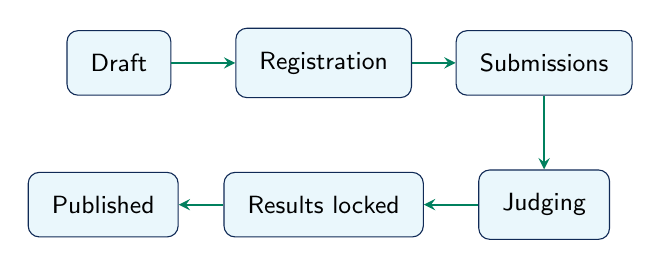
\begin{tikzpicture}[node distance=18mm, every node/.style={draw=DeepBlue,rounded corners,fill=PaleBlue,inner sep=3mm,font=\small}, >=stealth]
  \node (draft) {Draft};
  \node (reg) [right of=draft,xshift=8mm] {Registration};
  \node (submit) [right of=reg,xshift=10mm] {Submissions};
  \node (judge) [below of=submit] {Judging};
  \node (results) [left of=judge,xshift=-10mm] {Results locked};
  \node (published) [left of=results,xshift=-10mm] {Published};
  \draw[->,thick,Electric!60!black] (draft)--(reg);
  \draw[->,thick,Electric!60!black] (reg)--(submit);
  \draw[->,thick,Electric!60!black] (submit)--(judge);
  \draw[->,thick,Electric!60!black] (judge)--(results);
  \draw[->,thick,Electric!60!black] (results)--(published);
\end{tikzpicture}
\end{center}

The database timestamps, not frontend timers, should decide whether a transition or action is permitted.

\subsection{Weighted rubric calculation}

If criterion $k$ has weight $w_k$ and a judge gives project $i$ score $x_{ik}$, a transparent weighted score is:

\[
S_i = \frac{\sum_k w_k x_{ik}}{\sum_k w_k}.
\]

The implementation should document scale direction, missing criteria, rounding, whether comments are mandatory, whether a submitted review can be reopened, and whether weights may change after judging starts.

\subsection{Cross-judge normalization}

The deck requires cross-judge normalization but deliberately does not mandate an algorithm. The team must choose, implement, and defend one. A common demonstration method is judge-wise standardization:

\[
z_{ij}=\frac{s_{ij}-\mu_j}{\sigma_j},
\]

where $s_{ij}$ is judge $j$'s score for project $i$, and $\mu_j$ and $\sigma_j$ are that judge's mean and standard deviation. Project-level normalized values can then be aggregated.

This simple method exposes an important fixture edge case: the judge who scored every project identically has $\sigma_j=0$. The system must define a policy rather than divide by zero. Possible defensible policies include treating those normalized contributions as neutral, excluding them with an audit note, or falling back to a centered-but-unscaled value. Whatever the choice, it must be documented.

Other defensible approaches include rank/percentile transforms, robust centering and scaling, calibration against overlapping assignments, or a statistical model. The strongest submission shows both raw and normalized output and explains whether normalization changes the ordering.

\subsection{Assignment strategy}

A defensible strategy should discuss:

\begin{itemize}
  \item the desired number of judges per project;
  \item balancing workload across judges;
  \item track expertise and conflicts of interest;
  \item overlap between judges to support calibration;
  \item reassignment when a review batch remains incomplete; and
  \item the point at which assignments become immutable or auditable.
\end{itemize}

\subsection{CSV export}

At minimum, the required route must produce valid CSV\@. A useful export normally includes stable identifiers, project metadata, track, assignment status, raw criterion scores, criterion weights, raw aggregate, normalized aggregate, ranking, and timestamps. Sensitive data should not be included merely because an organizer export route exists; the schema and access policy belong in \texttt{DATA-MODEL.md}.

\subsection{Tier 3 abuse controls}

For community voting, a practical threat model should consider:

\begin{itemize}
  \item multiple accounts controlled by one person;
  \item scripted or high-rate votes;
  \item coordinated ballot stuffing;
  \item order and position bias;
  \item voting after the deadline;
  \item early result leakage; and
  \item administrators or judges changing records without a trace.
\end{itemize}

Rate limiting, identity requirements, randomized ordering, immutable event timestamps, hidden counts, anomaly flags, and append-only audit records are possible controls. The threat-model bonus explicitly permits honest disclosure of attacks the system does not stop.

\subsection{Tier 4 API and webhooks}

If pursuing API First or Tier 4, use the same authorization service for UI and API actions. Document endpoints through OpenAPI, version the API, define webhook signatures and retry behavior, and ensure bulk operations preserve the same validation and auditing as single-record actions.

% -----------------------------------------------------------------------------
\section{A risk-aware 72-hour execution plan}

\advisory\par


The following sequence follows the competition's scoring incentives rather than maximizing the number of visible features.

\begin{tabularx}{\linewidth}{@{}L{29mm}L{37mm}Y@{}}
\toprule
\textbf{Elapsed time} & \textbf{Focus} & \textbf{Exit condition}\\
\midrule
Hours 0--6 & Foundation & Compose stack starts offline; schema, migrations, seed, and four auth headers work\\
Hours 6--20 & Tier 1 & Public gallery, fixture projects, teams/submissions, and closed-event enforcement pass\\
Hours 20--40 & Tier 2 security and flow & Assignments, weighted scoring, own-score access, peer denial, and participant denial work\\
Hours 40--52 & Normalization and export & Method handles fixture edge cases; CSV and progress dashboard work\\
Hours 52--60 & Documentation & README, architecture, data model, and judging method match the implementation\\
Hours 60--66 & One differentiator & Complete one chosen bonus or a coherent T3 feature set\\
Hours 66--70 & Verification & Fresh offline setup, repeated checker runs, committed acceptance report\\
Hours 70--72 & Submission & Five-minute lifecycle demo, honest limits, final code freeze\\
\bottomrule
\end{tabularx}

% -----------------------------------------------------------------------------
\section{Final compliance checklist}

\subsection{Gate and local operation}

\begin{itemize}
  \item[\checkbox] Public repository uses an OSI-approved license.
  \item[\checkbox] A clean machine can run the product with \texttt{docker compose up}.
  \item[\checkbox] Startup and core workflows do not require network access.
  \item[\checkbox] Shared fixtures load deterministically, including awkward cases.
  \item[\checkbox] The fixture event preserves its own \texttt{submissions\_close} value.
\end{itemize}

\subsection{Tier 1}

\begin{itemize}
  \item[\checkbox] Authentication and roles work beyond a login screen.
  \item[\checkbox] Events and teams can be created or managed.
  \item[\checkbox] Project submission works before the deadline.
  \item[\checkbox] Submission is refused after the deadline.
  \item[\checkbox] The public gallery is reachable without authentication.
  \item[\checkbox] Fixture projects appear in the gallery.
\end{itemize}

\subsection{Tier 2}

\begin{itemize}
  \item[\checkbox] Judges can be invited and assigned.
  \item[\checkbox] The scoring rubric applies criterion weights.
  \item[\checkbox] Judges can access their own scores.
  \item[\checkbox] \texttt{judge\_b} receives \texttt{401} or \texttt{403} for \texttt{judge\_a}'s scores.
  \item[\checkbox] Participants are blocked from judge-only functionality.
  \item[\checkbox] Judging progress is visible.
  \item[\checkbox] Cross-judge normalization is implemented and documented.
  \item[\checkbox] CSV export works.
\end{itemize}

\subsection{Submission artifacts}

\begin{itemize}
  \item[\checkbox] \texttt{.dogfood.toml} contains working routes, headers, and honest claims.
  \item[\checkbox] \texttt{acceptance-report.txt} contains the actual latest checker output.
  \item[\checkbox] \texttt{README.md} documents operation and limitations.
  \item[\checkbox] \texttt{ARCHITECTURE.md} explains the system and design choices.
  \item[\checkbox] \texttt{DATA-MODEL.md} explains schema and data movement.
  \item[\checkbox] \texttt{JUDGING.md} defends assignment, scoring, and normalization.
  \item[\checkbox] The five-minute video demonstrates one full event lifecycle.
\end{itemize}

% -----------------------------------------------------------------------------
\section{Known ambiguities and boundaries of the brief}

The following details are not fully specified in the kickoff deck and should be resolved by inspecting the published specification and checker or by asking organizers:

\begin{itemize}
  \item The mission says ``ten stages'' but names nine; event creation is only an inferred tenth stage.
  \item The normalization algorithm is intentionally left open, although normalization itself is required.
  \item Route names, framework, database, and login mechanism are unrestricted, subject to local/offline operation.
  \item Only the peer-score denial slide explicitly mandates exact HTTP outcomes: \texttt{401} or \texttt{403}. Other precise checker assertions live in \texttt{run.py}.
  \item Tiers 3 and 4 are manually judged, and the slides do not publish a detailed point-by-point manual test protocol.
  \item MIT and Apache-2.0 are preferred, while the binding licensing requirement is an OSI-approved license.
  \item The slides do not state whether prize categories may be won simultaneously.
  \item The exact definition of ``verifiable judge records'' is not provided in the deck.
\end{itemize}

Recognizing these boundaries is part of honest delivery. The correct response is to inspect the authoritative files and document chosen interpretations, not to conceal uncertainty.

% -----------------------------------------------------------------------------
\section{Requirement traceability index}

\small
\begin{longtable}{@{}L{12mm}L{51mm}L{31mm}L{65mm}@{}}
\toprule
\textbf{Slide} & \textbf{Subject} & \textbf{Verification} & \textbf{Handbook coverage}\\
\midrule
\endhead%
1 & Event identity, dates, format, cost, prize pool & Administrative & Executive understanding; timeline; prizes\\
2 & Industry problem statement & Narrative evaluation & Problem statement\\
3 & Complete product mission and offline startup & Demo and operation & Mission; architecture; checklist\\
4 & Four-tier ladder & Gate, machine, and manual judging & Four-tier ladder\\
5 & Seven acceptance checks & Automated & Acceptance checker\\
6 & \texttt{.dogfood.toml} contract & Automated configuration & Acceptance checker configuration\\
7 & Shared fixtures and edge cases & Seed inspection and checker & Shared fixture dataset\\
8 & Judge-score isolation & Automated, exact denial outcome & Critical authorization requirement\\
9 & Nine submission artifacts & Submission review & Submission package\\
10 & 40/25/20/15 scoring & Weighted judging & Scoring model\\
11 & Four bonus challenges & Tie-break/manual & Bonus challenges\\
12 & Prize distribution & Administrative & Prize structure\\
13 & Teardown write-up & Separate review & Teardown write-up\\
14 & Ownership and adoption terms & Administrative & What happens to the winner\\
15 & UTC schedule & Deadline enforcement & Complete timeline\\
16 & Out-of-scope work & Eligibility/manual review & Explicitly out of scope\\
17 & Pre-start actions and official destinations & Participant preparation & Before starting\\
\bottomrule
\end{longtable}
\normalsize

\vfill
\begin{tcolorbox}[colback=Navy,colframe=Navy,arc=2mm,left=6mm,right=6mm,top=6mm,bottom=6mm]
\color{white}
{\Large\bfseries Final interpretation}\par
\vspace{2mm}
DOGFOOD rewards a small number of difficult qualities: correctness, secure isolation, transparent judging mathematics, operational simplicity, and honest engineering judgment. The strongest entry is not the one with the longest feature list. It is the one an organizer can start offline, understand, trust with private scores, and confidently use for the next real event.
\end{tcolorbox}

% -----------------------------------------------------------------------------
\section{Role-centered functional specification}

\advisory\par


The kickoff deck names capabilities, but an adoptable portal must connect them into coherent experiences for each actor. The workflows below make those expectations concrete without changing the official tier definitions.

\subsection{Organizer workflow}

\begin{longtable}{@{}L{31mm}L{42mm}L{84mm}@{}}
\toprule
\textbf{Phase} & \textbf{Organizer action} & \textbf{Observable outcome}\\
\midrule
\endhead%
Installation & Start the Compose stack on a disconnected laptop & Application, database, migrations, fixtures, and local assets become available without contacting an external service\\
Event setup & Create or inspect an event; define windows, tracks, eligibility, rubric, and visibility & The event has explicit server-side timestamps and a valid weighted rubric\\
Access setup & Create users or load fixtures; assign participant, judge, and organizer roles & The four checker identities are usable, and their auth headers are printed or otherwise easy to obtain\\
Submission period & Monitor registration, teams, and project completeness & Participants can submit only for their own teams and only inside the allowed window\\
Eligibility review & Flag duplicates or ineligible projects and record a reason & Only eligible projects proceed, while the original record and decision remain auditable\\
Judge setup & Invite judges, capture expertise/conflicts, and produce assignments & Every eligible project receives the intended coverage without assigning declared conflicts\\
Judging & Monitor completed, in-progress, and unstarted reviews & Incomplete batches are visible early enough for reassignment\\
Results calculation & Freeze inputs, run normalization, inspect raw versus adjusted results & The ranking is reproducible from a versioned method and immutable input snapshot\\
Publication & Release results only after the configured window & No public or participant endpoint leaks rankings before release\\
Closure & Export data, archive the event, and preserve documentation & The event can be audited, restored, or migrated without the original developer\\
\bottomrule
\end{longtable}

\subsection{Participant workflow}

A participant should be able to register, join or form a team, prepare a project, understand the deadline, submit, confirm the accepted state, and see the public gallery without receiving judge-only data. Submission ownership must follow authenticated team membership rather than a user-supplied team identifier.

Useful participant-facing states include \emph{draft}, \emph{submitted}, \emph{late/refused}, \emph{eligible}, \emph{ineligible}, and \emph{withdrawn}. If editing is allowed after an initial submission, the portal should state whether the deadline freezes the latest version, the first submitted version, or a separately confirmed final version.

\subsection{Judge workflow}

A judge should see only assigned projects and personal review records. A complete workflow is:

\begin{enumerate}
  \item authenticate as a judge;
  \item view assignment progress and conflict information;
  \item open an assigned project;
  \item score every required rubric criterion and add comments where required;
  \item save a draft without accidentally publishing a partial review;
  \item submit or finalize the review;
  \item see the judge's own completed scores; and
  \item remain unable to retrieve another judge's scores through either UI or API\@.
\end{enumerate}

The UI may hide peer scores, but the decisive rule is enforced by server-side ownership checks on every read and write.

\subsection{Public visitor workflow}

An unauthenticated visitor must be able to open the gallery and see the shared fixture projects. At Tier 3, the visitor may also vote or comment subject to the platform's identity and abuse policy. Results and vote totals should remain unavailable until the relevant release window closes.

\begin{keybox}
\textbf{Recommended invariant:} every protected action should be expressible as ``authenticated actor + event-scoped role + resource ownership + current event state''. Frontend visibility is presentation; this server-side decision is authorization.
\end{keybox}

% -----------------------------------------------------------------------------
\section{Judging integrity playbook and worked example}

\advisory\par


\subsection{Rubric definition and freezing}

Each criterion should have a stable identifier, label, description, numeric scale, weight, and ordering. Validate that weights are non-negative and that their total is meaningful. The portal should refuse to calculate a result from an empty rubric.

Once judging begins, editing a criterion or weight can retroactively change every score. A robust policy is to freeze the rubric or create a new rubric version, record who made the change, and recalculate through an explicit result run. Silent mutation damages reproducibility.

\subsection{Review lifecycle}

Suggested review states are \emph{unstarted}, \emph{draft}, \emph{submitted}, \emph{reopened}, and \emph{voided}. A submitted review should record its author and submission timestamp. Reopening or voiding it should require a reason and generate an audit event.

Missing criteria must have a defined treatment. Treating missing values as zero can unfairly penalize a project; silently averaging only completed criteria can reward incomplete judging. The product should either require completion or display an explicit provisional state.

\subsection{Worked normalization example}

Suppose two judges score three projects on the same aggregate scale. Judge 1 uses a relatively narrow, descending scale; Judge 2 uses a higher and wider scale.

\begin{center}
\begin{tabular}{@{}lrrrr@{}}
\toprule
\textbf{Project} & \textbf{Judge 1 raw} & \textbf{Judge 2 raw} & \textbf{Raw average} & \textbf{Raw rank}\\
\midrule
Alpha & 90 & 70 & 80.0 & 3\\
Beta  & 80 & 95 & 87.5 & 1\\
Gamma & 70 & 100 & 85.0 & 2\\
\bottomrule
\end{tabular}
\end{center}

Using population standardization within each judge gives approximately:

\begin{center}
\begin{tabular}{@{}lrrrr@{}}
\toprule
\textbf{Project} & \textbf{Judge 1 $z$} & \textbf{Judge 2 $z$} & \textbf{Mean $z$} & \textbf{Normalized rank}\\
\midrule
Alpha & 1.225 & -1.397 & -0.086 & 2\\
Beta  & 0.000 &  0.508 &  0.254 & 1\\
Gamma & -1.225 & 0.889 & -0.168 & 3\\
\bottomrule
\end{tabular}
\end{center}

The example changes the order of Alpha and Gamma. That does not prove standardization is universally correct; it demonstrates why the method must be visible and defended. A third judge who gives all three projects 75 has zero variance. The system must apply its documented zero-variance policy and report that treatment in the result run.

\subsection{Result-run provenance}

A reproducible normalization run should retain:

\begin{itemize}
  \item the event and rubric version;
  \item the set of included projects, assignments, and submitted reviews;
  \item the algorithm name and version;
  \item parameters, missing-data rules, and zero-variance rules;
  \item the actor who initiated the run and its timestamp;
  \item raw aggregates, normalized values, tie handling, and final ordering; and
  \item warnings such as incomplete batches or excluded records.
\end{itemize}

\subsection{Ties and incomplete judging}

Define ties before results are calculated. Possible policies include shared rank, deterministic secondary criteria, additional judging, or an explicitly documented tie-break bonus. Do not use an opaque database ordering as an accidental tie-break.

If judging is incomplete, the portal should either prevent final publication or label the result provisional. The two intentionally unfinished fixture batches make this behavior visible to evaluators.

% -----------------------------------------------------------------------------
\section{Security and threat model}

\advisory\par


\begin{longtable}{@{}L{31mm}L{38mm}L{43mm}L{46mm}@{}}
\toprule
\textbf{Asset} & \textbf{Threat} & \textbf{Primary control} & \textbf{Evidence to demonstrate}\\
\midrule
\endhead%
Judge scores & One judge reads a peer's scores & Server-side event role and record-ownership checks & Request as \texttt{judge\_b} for \texttt{judge\_a}; receive 401 or 403\\
Judge scores & Participant accesses judging routes & Deny participant role before querying data & Checker participant-blocked result plus manual API request\\
Submission window & Client clock or crafted request bypasses deadline & Compare authoritative server time with stored event timestamp & Post after \texttt{submissions\_close}; observe refusal and unchanged database\\
Project ownership & Participant edits another team's project & Team membership and resource ownership validation & Change project identifier while authenticated as another team\\
Results & Early ranking disclosure & Release-state checks on every result endpoint and export & Request results before release through UI, API, CSV, and embed routes\\
Community vote & Ballot stuffing or scripted voting & Identity policy, rate controls, deduplication signals, and audit events & Repeated vote attempts produce a visible, reviewable outcome\\
Administrative actions & Silent score or rubric changes & Append-only audit log and reasoned overrides & Show actor, old/new state, timestamp, and reason\\
Sessions & Guessable or leaked credentials & Random secrets, scoped cookies/tokens, and no fixture credentials in production & Explain generation, storage, expiration, and fixture-only boundaries\\
Webhook delivery & Forged callback or replay & Signature, timestamp, replay window, and event identifier & Verify invalid signature fails and repeated delivery is idempotent\\
CSV export & Spreadsheet formula injection & Escape or neutralize cells beginning with formula characters & Export hostile fixture text and inspect the resulting CSV\\
\bottomrule
\end{longtable}

\subsection{Audit-event minimum fields}

An audit event should include a stable event identifier, timestamp, authenticated actor, actor role, action, target type and ID, outcome, and relevant metadata. For sensitive changes, record a reason and an old/new summary. Avoid logging passwords, session tokens, or unnecessary personal data.

Audit records are useful only if ordinary users cannot rewrite them. If full immutability is impractical in 72 hours, document who can delete them and what residual risk remains.

\subsection{Failure behavior}

Authorization failures should return consistent 401/403 responses without revealing whether a protected record exists. Validation failures should identify correctable input problems. Unexpected failures should not expose stack traces, secrets, database queries, or other users' data.

% -----------------------------------------------------------------------------
\section{API, webhook, and data-exchange blueprint}

\advisory\par


The deck allows arbitrary routes; the table below is a suggested resource-oriented surface, not a checker contract.

\begin{longtable}{@{}L{54mm}L{31mm}L{73mm}@{}}
\toprule
\textbf{Example route} & \textbf{Primary role} & \textbf{Purpose}\\
\midrule
\endhead%
\texttt{GET /projects} & Public & Public gallery and fixture visibility\\
\texttt{POST /events/:id/projects} & Participant & Create a team-owned project inside the submission window\\
\texttt{POST /events/:id/submit} & Participant & Finalize or submit the project, subject to deadline and eligibility\\
\texttt{GET /judge/assignments} & Judge & List only the authenticated judge's assignments\\
\texttt{GET /judge/scores} & Judge & Retrieve only the authenticated judge's score records\\
\texttt{PUT /judge/reviews/:id} & Judge & Save or submit an authorized review\\
\texttt{GET /organizer/progress} & Organizer & Inspect assignment and completion progress\\
\texttt{POST /organizer/normalizations} & Organizer & Execute a versioned normalization run\\
\texttt{POST /organizer/results/publish} & Organizer & Publish results after release requirements are met\\
\texttt{GET /api/export.csv} & Organizer/checker & Produce the required CSV export\\
\bottomrule
\end{longtable}

\subsection{API properties}

If pursuing Tier 4 or API First, document:

\begin{itemize}
  \item authentication format and event-scoped authorization;
  \item request/response schemas and error structure;
  \item pagination, filtering, and stable ordering;
  \item idempotency for retried writes and bulk imports;
  \item API versioning and deprecation policy;
  \item rate limits where appropriate; and
  \item an OpenAPI document covering every UI action.
\end{itemize}

\subsection{Suggested webhook events}

Useful events include:

\begin{itemize}
  \item \texttt{project.submitted};
  \item \texttt{project.eligibility\_changed};
  \item \texttt{assignment.created};
  \item \texttt{review.submitted};
  \item \texttt{judging.completed}; and
  \item \texttt{results.published}.
\end{itemize}

Each delivery should have a unique ID, event type, creation timestamp, versioned payload, and signature. Retrying the same delivery must not duplicate downstream actions.

\subsection{CSV contract}

The checker route should respond with a CSV media type and syntactically valid rows. For human and machine use, prefer UTF-8, a stable header row, stable identifiers, consistent timestamp format, explicit blank/missing semantics, and deterministic ordering. Document whether the file contains one row per project, assignment, review, or criterion score.

For reproducibility, an organizer export may be split into several files: projects, teams, users/roles, assignments, criterion scores, normalized results, and audit events. The acceptance checker requires only that its configured CSV export work; richer export is an adoptability feature.

% -----------------------------------------------------------------------------
\section{Offline operations and recovery runbook}

\advisory\par


\subsection{Fresh-machine verification}

Before submission, test the exact evaluator path:

\begin{enumerate}
  \item use a clean checkout without local developer state;
  \item disconnect networking or block outbound access;
  \item run \texttt{docker compose up};
  \item wait only for documented health checks, migrations, and seed completion;
  \item capture the printed organizer, two judge, and participant headers;
  \item fill in \texttt{.dogfood.toml};
  \item run the checker; and
  \item stop and restart the stack to confirm persistence and idempotent startup.
\end{enumerate}

Images, packages, fonts, JavaScript bundles, database extensions, and migrations must already be present locally. A page that loads but waits on a remote CDN does not meet the spirit of network-off operation.

\subsection{Backups and restoration}

An operator should know which volume or files contain database state and uploaded assets. Document a backup command, a restoration command, and whether backups are consistent while the application is running. Test one restoration rather than documenting an unverified procedure.

\subsection{Time and timezone}

Store authoritative instants in UTC and render them with an explicit timezone. Deadline comparisons should occur on the server. The UI should show the event timezone or UTC clearly so participants do not infer a local time incorrectly.

\subsection{Operational visibility}

A minimal health endpoint should distinguish application availability from database readiness. Logs should identify migration, seed, authentication, assignment, export, and normalization failures without exposing secrets. Organizer dashboards should surface actionable states such as incomplete batches and failed webhook deliveries.

\subsection{Safe restart behavior}

Repeated startup should not duplicate the 40 projects, 30 judges, 8 tracks, scores, or fixture users. Seed operations should use stable identifiers or an explicit reset mode. Destructive reset behavior must be opt-in and clearly labeled.

% -----------------------------------------------------------------------------
\section{Verification strategy and five-minute demo storyboard}

\advisory\par


\subsection{Minimum high-value tests}

\begin{longtable}{@{}L{37mm}L{52mm}L{69mm}@{}}
\toprule
\textbf{Test family} & \textbf{Example} & \textbf{Risk covered}\\
\midrule
\endhead%
Startup & Fresh offline Compose boot with empty volumes & Adoption failure and hidden cloud dependency\\
Seed & Run seed twice and count fixture records & Duplicate data and non-repeatable evaluation\\
Deadline & Submit one second before and at/after close & Boundary errors and client-clock bypass\\
Authorization & Cross every role with every protected route & Peer-score and participant leakage\\
Ownership & Change team/project/judge identifiers in requests & Insecure direct object reference\\
Rubric & Invalid weights, boundary scores, missing criteria & Incorrect aggregates and weak validation\\
Normalization & Constant judge, missing reviews, ranking change & Divide-by-zero and unexplained results\\
Export & Parse CSV containing commas, quotes, newlines, and formula-like text & Broken interchange and spreadsheet injection\\
Publication & Request results through all surfaces before release & Premature disclosure\\
Recovery & Restart and restore a backup & Data loss and unrecoverable operation\\
\bottomrule
\end{longtable}

\subsection{Five-minute demo storyboard}

\begin{tabularx}{\linewidth}{@{}L{22mm}L{49mm}Y@{}}
\toprule
\textbf{Time} & \textbf{Action} & \textbf{Evidence delivered}\\
\midrule
0:00--0:30 & Start with the product claim and architecture & One product, offline, intended tier, and honest limitations\\
0:30--1:00 & Show startup and fixture gallery & Compose operation, public access, and seeded projects\\
1:00--1:35 & Demonstrate team submission and deadline refusal & Working participant flow and server-side event state\\
1:35--2:15 & Show organizer assignment and progress & Multiple judges, batches, and incomplete-review visibility\\
2:15--3:00 & Enter weighted judge scores & Rubric behavior and personal review access\\
3:00--3:30 & Attempt peer-score and participant access & Visible 401/403 role isolation at the backend\\
3:30--4:10 & Run normalization and compare raw/results & Defended method, fixture edge case, and ranking provenance\\
4:10--4:35 & Export CSV and show result controls & Portability and controlled publication\\
4:35--5:00 & Show checker output and documentation & Evidence, honest gaps, and immediate adoptability\\
\bottomrule
\end{tabularx}

The demo should not spend most of its time on slides. The application, network panel or HTTP client, checker output, and relevant documents provide stronger evidence.

% -----------------------------------------------------------------------------
\section{Documentation blueprint and decision record}

\advisory\par


\subsection{README structure}

Include the product's purpose, claimed tiers, screenshots or a concise feature list, prerequisites, exact offline startup steps, fixture credentials/headers, checker invocation, known limitations, license, and links to the deeper technical documents.

\subsection{Architecture document}

Explain components, trust boundaries, runtime containers, request flow, authorization placement, persistence, seed behavior, result calculation, exports, and major tradeoffs. A diagram should agree with the Compose file and deployed code.

\subsection{Data-model document}

Describe entities, keys, relationships, lifecycle states, timestamp/timezone policy, migrations, deletion policy, fixture import, CSV/bulk export, and how duplicate submissions and incomplete reviews are represented.

\subsection{Judging document}

State assignment objectives, conflict handling, rubric and weighting mathematics, missing-score policy, normalization formula, zero-variance treatment, tie policy, incomplete-judging policy, publication conditions, and a worked raw-to-final example.

\subsection{Architecture decision record}

For each consequential choice, record the context, chosen option, alternatives considered, consequences, and whether the decision is reversible. High-value decisions include the authentication model, database, deadline semantics, duplicate policy, assignment algorithm, normalization method, audit design, and API versioning.

\begin{advicebox}
Documentation is strongest when it describes the software that actually exists. Update the documents after the final implementation decisions, and preserve known weaknesses rather than replacing them with aspirational language.
\end{advicebox}
\end{document}